\subsection{泊松过程的定义}

\begin{definition}[计数过程]
    若随机变量 $N(t)$ 表示时间段 $[0,t]$ 内某事件发生的次数, 则称 $\{N(t),t\geq 0\}$ 是一个计数过程, 若
    \begin{enumerate}
        \item $N(t)\geq 0$ 取整数值
        \item 若 $s<t$, 则 $N(s)\leq N(t)$, 且 $N(t)-N(s)$ 表示时间段 $(s,t]$ 内事件的发生次数
    \end{enumerate}
\end{definition}

\begin{definition}[泊松过程I]\label{def:counting-process-I}
    称一个计数过程 $\{N(t),t\geq 0\}$ 是一个带有参数/速率 $\lambda(\lambda>0)$ 的泊松过程, 若
    \begin{enumerate}
        \item $N(0)=0$, 即 $\PP(N(0)=0)=1$
        \item (独立增量) $\forall 0\leq t_1<t_2<\cdots<t_n$, 有
        \[
        N(t_2)-N(t_1),\cdots,N(t_n)-N(t_{n-1})
        \]
        相互独立
        \item $\forall t>0,s\geq 0, N(t+s)-N(s)\sim \Poi(\lambda t)$
    \end{enumerate}
\end{definition}

\begin{property}
由 Def \ref{def:counting-process-I} (3) 易知, $(N(t))_{t\geq 0}$ 具有平稳增量.
\[
N(t+s)-N(s)\xlongequal{(d)} N(t)-N(0)\xlongequal{(d)}N(t)\sim \Poi(\lambda t)
\]
注: $\EE N(t)=\lambda t\Rightarrow \lambda=\EE N(t)/t$ 过程的速率
\end{property}

\begin{property}[Durrett, Lem 2.5]
对固定 $s\geq 0, \{N(t+s)-N(s),t\geq 0\}$ 仍是一个带有速率 $\lambda$ 的Poisson过程, 且 $N(t+s)-N(s)\ind N(r), \forall 0\leq r\leq s,t\geq 0$
\end{property}

\begin{definition}[泊松过程II: 到达时间间隔]\label{def:poi-2}
    令 $\tau_1,\tau_2,\cdots$ 为一列独立同分布的随机变量, $\tau_1\sim \EXP(\lambda)$,
    \[
    T_n=\begin{cases}
        \sum_{k=1}^n\tau_k & n\geq 1\\
        0 & n=0
    \end{cases}
    \]
    $N(t)=\max\{n|T_n\leq t\}$, 则称 $\{N(t),t\geq 0\}$ 为带有速率 $\lambda$ 的Poisson过程
    
    注: ``无穷小定义'', 见 Sheldon Ross 随机过程\cite{ross1995stochastic}.
\end{definition}
注:
\begin{enumerate}
    \item $T_n(n\geq 1)$: 第 $n$ 个顾客的到店时刻
    \item $\tau_n(n\geq 1)$: 第 $n$ 个和第 $n-1$ 个顾客的到店时间间隔
    \item $N(t)$: $t$ 时刻之前到达的顾客总数
\end{enumerate}
\begin{figure}[H]
    \centering
    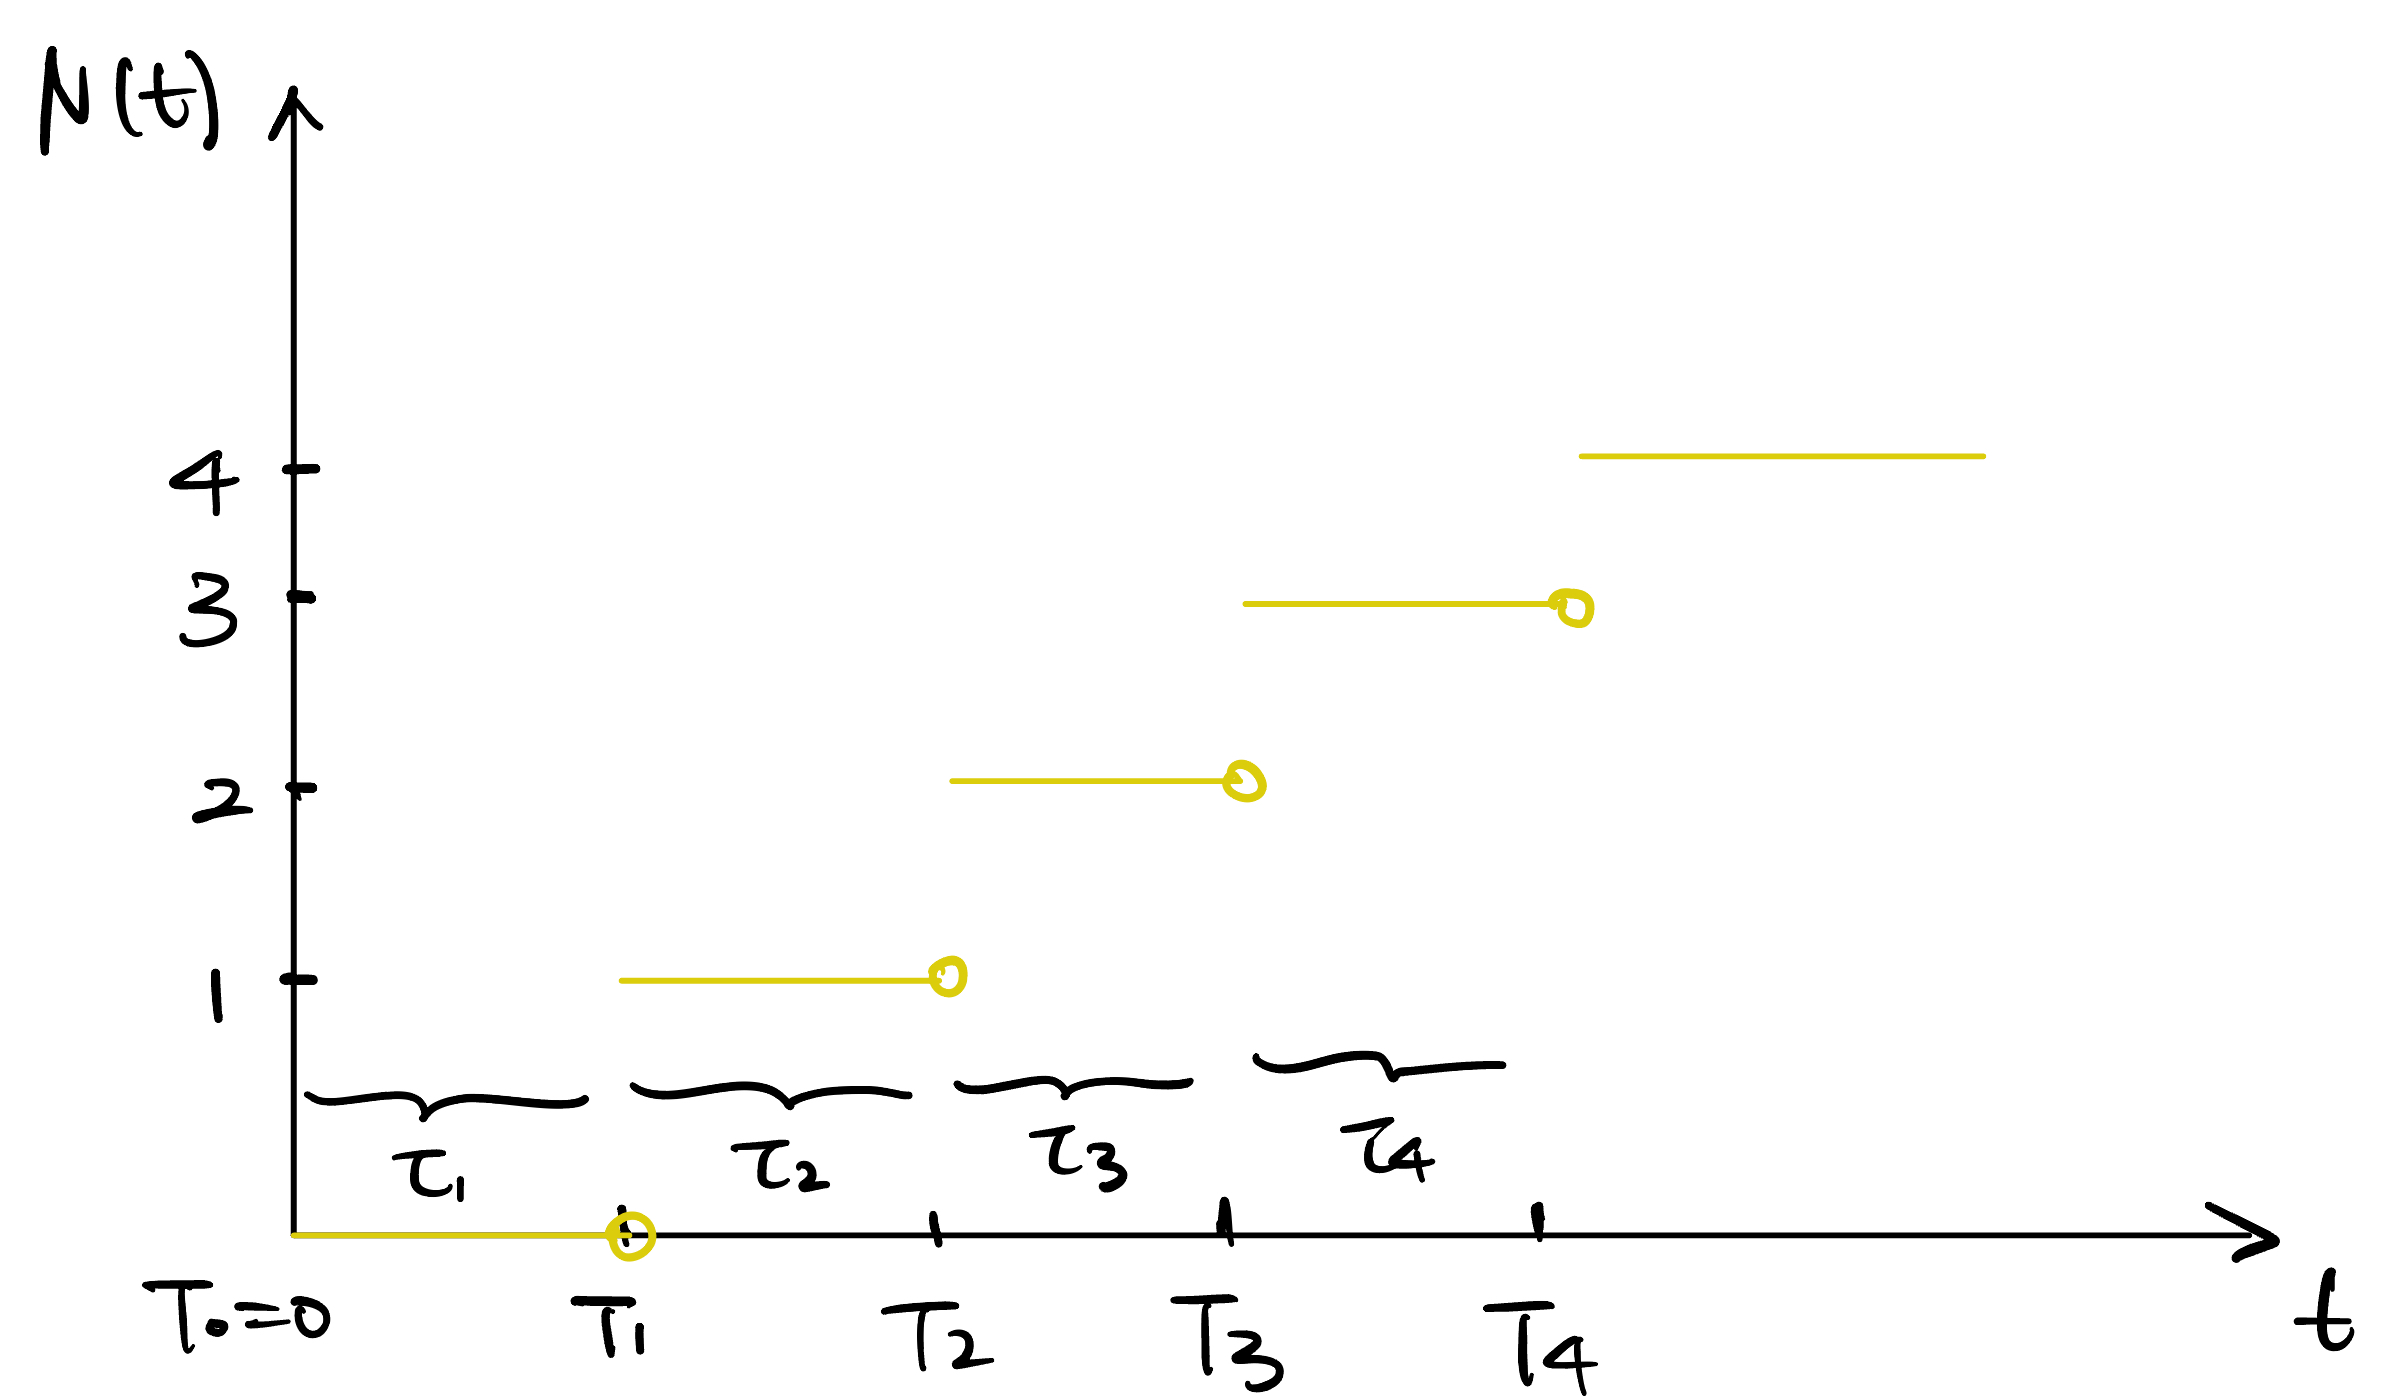
\includegraphics[width=0.65\textwidth]{figures/arrival.png}
    \caption{Arrival}
\end{figure}
注意 $T_1,T_2,\cdots$ 是随机的
\begin{enumerate}
    \item $n\geq 1, \tau_n=T_n-T_{n-1}\sim \EXP(\lambda), T_n\sim\Gamma(n,\lambda)$
    \item $\{N(t)=n\}=\{T_n\leq t< T_{n+1}\}$
    \item $\{N(t)\geq n\}=\{t\geq T_n\}$
    \item $\{N(t)<n\}=\{t<T_n\}$
\end{enumerate}

\begin{theorem}
    两种定义是等价的, 即 Def \ref{def:counting-process-I} $\iff$ Def \ref{def:poi-2}
\end{theorem}

\begin{proposition}
    Def \ref{def:poi-2} $\Rightarrow$ Def \ref{def:counting-process-I}
\end{proposition}

\begin{proof}
\begin{enumerate}
    \item $\{N(0)=0\}=\{T_1>0\}=\{\tau_1>0\}\Rightarrow \PP(N(0)=0)=\PP(\tau_1>0)=1$
    
    先引入下面引理.
    \begin{figure}[H]
        \centering
        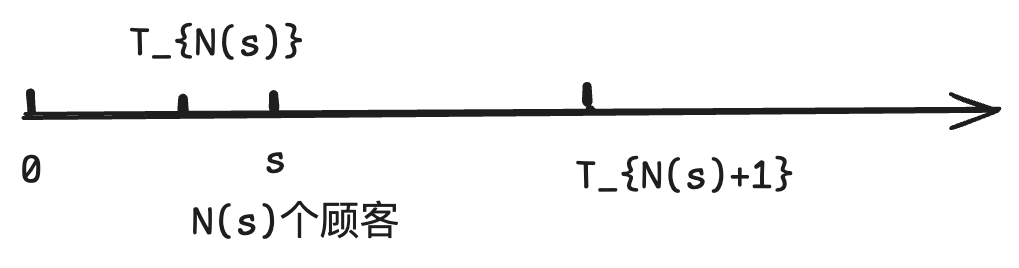
\includegraphics[width=0.35\textwidth]{figures/lem2-5.png}
        \caption{固定起始时间$s$}
        \label{fig:fixed-s}
    \end{figure}
\begin{lemma}[Lem 2.5']\label{lem:2.5}
    对固定$s\geq 0$ (图 \ref{fig:fixed-s}),
    令 $\tau_1^s:=T_{N(s)+1}-s$. $\tau_n^s:=\tau_{N(s)+n}, n\geq 2$.
    \[
    T_n^s:=\begin{cases}
        \sum_{k=1}^n\tau_k^s & n\geq 1\\
        0 & n=0
    \end{cases}
    \]
    $N^s(t):=\max\{n|T_n^s\leq t\}$. 则
    \begin{enumerate}
        \item $N^s(t)=N(t+s)-N(s)$
        \item $\forall k\geq 1, (\tau_1^s,\cdots,\tau_k^s)\ind N(s)$, 即 $\tau_k^s=\tau_k\sim \EXP(\lambda)$, $\tau_1^s, \tau_2^s, \cdots$ 相互独立
        \item $\{N^s(t)=N(t+s)-N(s),t\geq 0\}$ 为带有速率 $\lambda$ 的泊松过程, 且 $N(t+s)-N(s)\ind N(r), \forall 0\leq r\leq s,t\geq 0$
    \end{enumerate}
\end{lemma}
    \item (独立增量) 由 Lem \ref{lem:2.5} (c) 及数学归纳法
    
$n=2$, 对 $0=t_0\leq t_1<t_2$, 有 $N(t_2)-N(t_1)\ind N(t_1)=N(t_1)-N(t_0)$.
    
$n=k$, 假设对 $0=t_0\leq t_1<t_2<\cdots<t_n$, 有 $N(t_k)-N(t_{k-1}),\cdots,N(t_1)-N(t_0)$ 相互独立. 考虑 $n=k+1$, 对于第 $k+1$ 个增量 $N(t_{k+1})-N(t_k)$, 由 Lem \ref{lem:2.5} (c), 令 $s=t_k, N^{s}(t_{k+1}-t_k)\ind N(r), \forall r\leq t_k$, 因此由 Thm \ref{thm:1.3}, $N^{s}(t_{k+1}-t_k)\ind \sigma(\bigcup_{r\leq t_k}N(r))$. $\forall 1\leq j\leq k, N^{s}(t_{k+1}-t_k)\ind (N(t_j)-N(t_{j-1}))$. 又因 $\forall 1\leq j\leq k, N(t_j)-N(t_{j-1})$ 相互独立, 则 $\forall 1\leq j\leq k+1, N(t_j)-N(t_{j-1})$ 相互独立.
    \item 由 Lem \ref{lem:2.5} (a)(c) 知, 只需证 $N(t)\sim \Poi(\lambda t)$, 则有 $N(t+s)-N(s)\sim\Poi(\lambda t)$. 这是因为 Lem \ref{lem:2.5} (a)(c) 已经把 $N(t+s)-N(s)$ 表达为一个``从 $s$ 开始重新计时''的新泊松过程 $N^s(t)$, 而我们知道 $N^s(t)$ 的构造方式与原始的 $N(t)$ 完全一致, 只不过起点平移到了 $s$.
    \begin{enumerate}
        \item $\PP(N(t)=0)=\PP(T_1>t)=\PP(\tau_1>t)=e^{-\lambda t}(\lambda t)^0/(0!)$
        \item $n>0$ 时, 
        \[
        \begin{aligned}
            \PP(N(t)=n) &=\PP(T_n\leq t<T_{n+1})\\
            &=\PP(T_n\leq t<T_n+\tau_{n+1})\\
            &\xlongequal{T_n\ind \tau_{n+1}}\int_0^{+\infty}\PP(u\leq t<u+\tau_{n+1})f_{T_n}(u)du\\
            &=\int_0^{+\infty}\II_{\{u\leq t\}}\PP(\tau_{n+1}>t-u)f_{T_n}(u)du\\
            &=\int_0^t e^{-\lambda (t-u)}\lambda e^{-\lambda u}\frac{(\lambda u)^{n-1}}{(n-1)!}du\\
            &=\frac{\lambda^n e^{-\lambda t}}{(n-1)!}\int_0^t e^{\lambda u}\cdot e^{-\lambda u}u^{n-1}du\\
            &=\frac{\lambda^n e^{-\lambda t}}{(n-1)!}\cdot \frac{1}{n}\cdot u^n|_0^t=\frac{(\lambda t)^n e^{-\lambda t}}{n!}\sim \Poi(\lambda t)
        \end{aligned}
        \]
    \end{enumerate}
\end{enumerate}
\end{proof}

下面证明 Lem \ref{lem:2.5}.
\begin{proof}
\begin{enumerate}
    \item[(a)] 要证 $N^s(t)=N(t+s)-N(s)$. 
    
    $n\geq 1, T_n^s=T_{N(s)+1}-s+\tau_{N(s)+2}+\cdots +\tau_{N(s)+n}=T_{N(s)+n}-s, T_{N(s)}\leq s$
    \[
    \begin{aligned}
        N^s(t)&=\max\{n\geq 0|T_n^s\leq t\}\\
        &=\max\{n\geq 0|T_{N(s)+n}\leq t+s\}\\
        &\xlongequal{m=N(s)+n}\max\{m-N(s)\geq 0|T_m\leq t+s\}\\
        &=\max\{m\geq 0|T_m\leq t+s\}-N(s)\\
        &=N(t+s)-N(s)
    \end{aligned}
    \]
    \item[(b)] 要证明
    \begin{quote}
        $\forall k\geq 1$, \framebox{$(\tau_1^s,\cdots,\tau_k^s)\ind N(s)$}, 即 $\tau_k^s=\tau_k\sim \EXP(\lambda)$, $\tau_1^s, \tau_2^s, \cdots$ 相互独立
    \end{quote}
    实际上方框内的陈述更强, 目前无法证明, 所以只证后面的部分.
    \begin{enumerate}
        \item[(1)] $k=1$,
        \[
        \begin{aligned}
        \PP(\tau_1^s>t_1,N(s)=n) &=\PP(T_{N(s)+1}-s>t_1,N(s)=n)\\
        &=\PP(T_{n+1}>t_1+s,s\geq T_n)\\
        &=\PP(\tau_{n+1}>t_1+s-T_n, T_n\leq s)\\
        &\xlongequal{T_n\ind \tau_{n+1}}\int_0^{+\infty}\PP(\tau_{n+1}>t_1+s-u,u\leq s)f_{T_n}(u)du\\
        &=\int_0^{+\infty}\II_{\{u\leq s\}}\PP(\tau_{n+1}>t_1+s-u)f_{T_n}(u)du\\
        &\xlongequal{(*)}\int_0^{+\infty}\II_{\{u\leq s\}}\PP(\tau_{n+1}>s-u)f_{T_n}(u)du\cdot \PP(\tau_{n+1}>t_1)\\
        &=\PP(\tau_{n+1}>s-T_n,T_n\leq s)\PP(\tau_{n+1}>t_1)\\
        &=\PP(T_{n+1}>s\geq T_n)\PP(\tau_{n+1}>t_1)\\
        &=\PP(N(s)=n)\PP(\tau_{n+1}>t_1)
        \end{aligned}
        \]
        $(*)$ 处用了指数分布的无记忆性, 
        \[
        \begin{aligned}
				\PP(\tau_{n+1}>t_1+s-u)&=\PP(\tau_{n+1}>t_1+s-u|\tau_{n+1}>t_1)\cdot \PP(\tau_{n+1}>t)\\
				&=\PP(\tau_{n+1}>s-u)\cdot \PP(\tau_{n+1}>t)
				\end{aligned}
        \]
        最后关于 $n$ 求和, 
        \[
        \sum_{n\geq 0}\PP(\tau_1^s>t_1,N(s)=n)=\sum_{n\geq 0}\PP(N(s)=n)\PP(\tau_{n+1}>t_1)
        \]
        其中 $\LHS=\PP(\tau_1^s>t_1)$. 因为 $\PP(\tau_{n+1}>t_1)\xlongequal{iid}\PP(\tau_{1}>t_1)$, $\Rightarrow \RHS=\PP(\tau_{1}>t_1) \Rightarrow \tau_1^s\sim \EXP(\lambda)$. 代回, 得 $\PP(\tau_1>t_1)=\PP(\tau_1^s>t_1)$, 即 $\tau_1^s\ind N(s)$.

        注: $\PP(T_{n+1}-s>t|N(s)=n)=\PP(\tau_1^s>t|N(s)=n)=\PP(\tau_1>t)$. $\Rightarrow T_{n+1}-s\sim \EXP(\lambda)$ under $\PP(\cdot|N(t)=n)$.
        \item[(2)] $k\geq 2$时, 
        \[
        \begin{aligned}
            A_n &:=\{N(s)=n,\tau_1^s>t_1,\tau_2^s>t_2,\cdots, \tau_k^s>t_k\}\\
            &=\{T_n\leq s,T_{n+1}>t_1+s\}\cap \left\{\bigcap_{i=2}^k \{\tau_{n+2}>t_i\}\right\}
        \end{aligned}
        \]
        \[
        \begin{aligned}
            \PP(A_n) &=\PP(T_n\leq s, T_{n+1}>t_1+s)\prod_{i=2}^k \PP(\tau_{n+i}>t_i)\\
            &\xlongequal{k=1}\PP(N(s)=n)\PP(\tau_1>t_1)\prod_{i=2}^k\PP(\tau_{n+i}>t_i)
        \end{aligned}
        \]
        在概率测度意义下 $\tau_{n+i}\overset{(d)}{=}\tau_i$, 关于 $n$ 求和, $(\tau_1^s,\cdots,\tau_k^s)\overset{(d)}{=}(\tau_1,\cdots,\tau_k)$, 即 $\tau_1^s,\cdots,\tau_k^s$ 相互独立, 代回前式得 $(\tau_1^s,\cdots,\tau_k^s)\ind N(s)$.
        \item[(3)] 类似前面两步的技巧.
    \end{enumerate}
    \item[(c)] 不妨设 $0\leq t_1<\cdots<t_k$
    \[
    \begin{aligned}
        \{N^s(t_1)=m_1,\cdots,N^s(t_k)=m_k\} &=\{T_{m_1}^s\leq t_1< T_{m_1+1}^s,\cdots,T_{m_k}^s\leq t_k< T_{m_k+1}^s\}\\
        &=\left\{\sum_{i=1}^{m_1}\tau_i^s\leq t_1<\sum_{i=1}^{m_1+1}\tau_i^s,\cdots,\sum_{i=1}^{m_k}\tau_i^s\leq t_k<\sum_{i=1}^{m_k+1}\tau_i^s\right\}
    \end{aligned}
    \]
    由 (b), $\tau_i^s\sim \EXP(\lambda),\forall i\geq 0$. 由 Def \ref{def:poi-2}, $N^s(t_i),\forall i\geq 0$ 为速率 $\lambda$ 的泊松过程. 
\end{enumerate}
\end{proof}

\begin{proposition}
    Def \ref{def:counting-process-I} $\Rightarrow$ Def \ref{def:poi-2}
\end{proposition}

\begin{proof}
$\{N(t),t\geq 0\}$ 是计数过程, $T_n=\min\{t|N(t)\geq n\}, \tau_n=T_n-T_{n-1}$.
\begin{enumerate}
    \item $t\neq 0$, 
    \[
    N(t)=\sum_{n=1}^{\infty}\II_{\{N(t)\geq n\}}=\sum_{n=1}^{\infty}\II_{\{T_n\leq t\}}=\max\{n|T_n\leq t\}
    \]
    \item 下面只需证 $(\tau_k)_{k\geq 1}\overset{\text{iid}}{\sim}\EXP(\lambda)$
    \begin{enumerate}
        \item $k=1, \PP(\tau_1>t)=\PP(T_1>t)=\PP(N(t)=0)=e^{-\lambda t}(\lambda t)^0/(0!)=e^{-\lambda t}$, 故 $\tau_1\sim\EXP(\lambda)$.
        \item 考察 $(T_1,T_2), S=\{(x_1,x_2)\in \RR^2|0<x_1<x_2\}$. 设 $0<r_1<t_1<r_2<t_2$
        \begin{figure}[H]
            \centering
            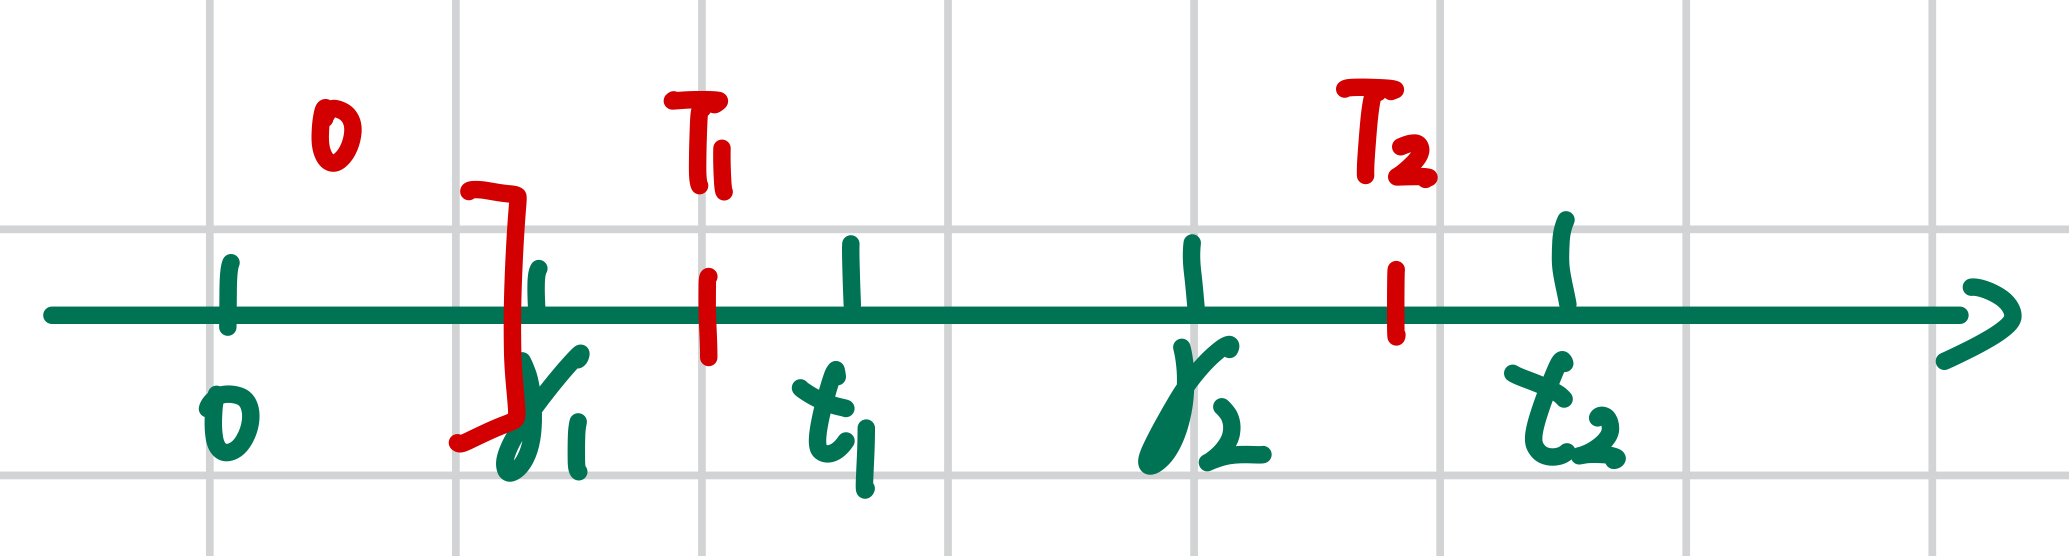
\includegraphics[width=0.35\textwidth]{figures/note-p102.png}
        \end{figure}
        \[
        \begin{aligned}
            &\PP(r_1\leq T_1<t_1,r_2\leq T_2<t_2) \\
            =&\PP(N(r_1)=0,N(r_2)-N(t_1)=0,N(t_1)-N(r_1)=1,N(t_2)-N(r_2)\geq 1)\\
            =&e^{-\lambda r_1}\cdot e^{-\lambda (r_2-t_1)}\cdot e^{-\lambda (t_1-r_1)}\cdot \frac{\lambda (t_1-r_1)}{1!}\cdot [1-e^{-\lambda (t_2-r_2)}]\\
            =&\lambda (t_1-r_1)[e^{-\lambda r_2}-e^{-\lambda t_2}]=\lambda\int_{r_1}^{t_1}dx_1\int_{r_2}^{t_2}\lambda e^{-\lambda x_2}dx_2
        \end{aligned}
        \]
        $N(t_2)-N(r_2)\geq 1$ 是因为要求第二个事件 $T_2$ 必须落在 $[r_2,t_2)$ 内, 但并不限制该区间内后续事件的数量. 联合密度函数 $\lambda^2 e^{-\lambda x_2}$ 在区域 $S$ (即 $0<x_1<x_2$) 上, 所以 $f_{(T_1,T_2)}(x_1,x_2)=\lambda^2 e^{-\lambda x_2}\II_{\{(x_1,x_2)\in S\}}$.
        \[
        \PP(\tau_1>t_1,\tau_2>t_2)=\PP(\tau_1>t_1,T_2-T_1>t_2)=\int_{x_1>t_1}\int_{x_2-x_1>t_2}\lambda^2 e^{-\lambda x_2}dx_2 dx_1=e^{-\lambda (t_1+t_2)}
        \]
        又 $\PP(\tau_1>t_1)=e^{-\lambda t_1}$, 所以 $\tau_2\sim \EXP(\lambda)$ 且 $\tau_1\ind \tau_2$. 对 $k\geq 3$ 同理.
    \end{enumerate}
\end{enumerate}
\end{proof}

\begin{definition}[Def \ref{def:counting-process-I} 推广, 非齐次的泊松过程]
    称计数过程 $\{N(t),t\geq 0\}$ 为一个速率为 $\lambda(r)$ 的非齐次泊松过程, 若
    \begin{enumerate}
        \item $N(0)=0$
        \item 独立增量性
        \item 增量的分布
        \[
        N(t+s)-N(s)\sim \Poi(\int_s^{t+s}\lambda(r)dr)
        \]
    \end{enumerate}
\end{definition}

\begin{proposition}
    非齐次泊松过程的到达间隔时间列 $\tau_1,\tau_2,\cdots$ 不再服从指数分布, 不再相互独立.
\end{proposition}
\begin{proof}
    同上计算联合分布即可.
\end{proof}
\newpage